\documentclass[USenglish,twocolumn]{article}
\usepackage{etex}
\usepackage[utf8]{inputenc}
\usepackage[big,online]{dgruyter}
\usepackage{hypernat}
\usepackage{tikz}
\usetikzlibrary{shapes,arrows}
\usepackage{pgfplots}
\usepackage{pgfplotstable}
\setcitestyle{numbers,square,comma,sort&compress}

\begin{document}

%%%--------------------------------------------%%%
%%% Please do not alter the following 7 lines: %%%
%%%--------------------------------------------%%%
	\articletype{Proceedings}
  \journalname{Current~Directions~in~Biomedical~Engineering}
  \journalyear{2015}
  \journalvolume{1}
  \journalissue{???}
  \startpage{1}
  %\aop
  \DOI{10.1515/bmt-XXXX}
%%%--------------------------------------------%%%

\title{On optimisation in HDR brachytherapy}
\runningtitle{On optimisation in HDR brachytherapy}
%\subtitle{Insert subtitle if needed}
\author[1]{Laurin Mordhorst}
\author[2]{Thobias Karthe}
\author[2]{Sebastian Elm}
\author[2]{Dawid Golebiewski} 
\author[2]{Malte Erik Schröder}
\runningauthor{Mordhorst, L.; Karthe, T.; Elm, S.; Golebiewski, D.; Schröder, M. E.}

\affil[1]{\protect\raggedright 
  TUHH,  e-mail: laurin.mordhorst@tuhh.de}
\affil[2]{\protect\raggedright 
  TUHH,  e-mail: thobias.karthe@tuhh.de, sebastian.elm@tuhh.de, dawid.golebiewski@tuhh.de, malte.schroeder@tuhh.de}
	

\abstract{Hallo na Please insert your abstract here. Remember that online
systems rely heavily on the content of titles and abstracts to
identify articles in electronic bibliographic databases and search
engines. We ask you to take great care in preparing the abstract.}

\keywords{Optimisation, Treatment planning, Brachytherapy, Genetic Algorithm, Simulated Annealing, Linear Programmin}

\maketitle

\section{Introduction} 

The aim of this article is to compare three different approaches in HDR-Brachytherapy treatment planning. The three analysed algorithms are linear programming, simulated annealing and genetic algorithms. The results are evaluated by analysing the conformity and homogeneity of the dose-distribution as well as runtime for different parameters.  

\section{Model description}
HDR brachytherapy consists of several radioactive sources being placed inside the patient's body by needles. These sources will eradiate into the surrounding tissues, treating tumor cells and other critical volumes. Therefore, it relies heavily on optimal algorithms to determine the dwell times for certain, predefined goals. \\
The body is represented by an equidistant grid of voxels, defining the single body cell type. The seeds are randomly positioned within the tumor voxels. Hence, the dosis in a voxel is calculated as a sum of each seed by evaluating the dose-function up to a fixed limit, where the influence gets negligible.

\section{Genetic Algorithm}
The Genetic Algorithm as introduced in \citep{1} has a lot of parameters which are described in the following. 

\subsection{Parameters}

\subsubsection{Weights}
The Fitness-Function used in the Genetic Algorithm is implemented as a sum of squared distances. But every tissue type can be weighted with an individual coefficent. 

\subsubsection{Probabilities} 
There are two important probabilites within the algorithm. The first one is the crossover rate. It describes how likely it is for two individuals to reproduce. The second one is the mutation rate. It describes, analogous to the crossover rate, the probability for an individual to perform a mutation. 

\subsubsection{Scaling and Accuracy}
The fitness-function for the given optimisation problem has very high computational complexity. Hence two scaling parameters are introduced to achieve shorter runtimes. The challenge here is to find a compromise between good accuracy for the optimisation and practicable runtimes.\\ The first parameter is called the \textit{treatment range}. It chooses the range around the PTV which shall be evaluated by the algorithm. The second parameter is a simple scaling value which defines that just every  $n^{th}$ voxel is evaluated. Within the treatment range of course.


\subsection{Results}


\subsubsection{Weights}
It seems hard to examine a specific sets of weights, that is applicable to any type of patients. The experiment has shown, that a higher weighted treatment has a much higher runtime and the convergency decreases.  

\subsubsection{Probabilities} 
The results have shown, that a high mutation rate leads to a very low tumor coverage. Furthermore the algorithm often doesn't converges, because the changes of the individuals accure too often. A stable state becomes less likely. \\ For the crossover rate the results showed, that the value should be between 0.7 and 0.9.

\subsubsection{Scaling and Accuracy}
The dose distribution of a radioactive seed shows that the dose at a radius of 10 cm is negligible small. So any treatment range higher than 10 cm wouldn't lead to better results anyway. (TODO: which range is acceptable)

\section{Linear Programming}
In Linear Programming a objective function and constraints are used to compute the optimal solution, as described in \citep{2}.

\subsection{Objective function and Constraints}
The objective function sums up the dose for every organ at risk voxel and is then minimized. The constraints restrict the optimization so that the level of radiation in the tumor does not fall under a fixed value. The contraints can be relaxed to lower the level of radiation in the surrounding organs at the cost of lowering the radiation at the border of the tumor.

\subsection{Results}
As shown in tabel \ref{table:LP_results50} and \ref{table:LP_results100}, the relaxation of the PTV increases the conformality, while letting the coverage of the PTV drop. 
		\begin{table}[h]
			\centering		
		 	\caption{LP 50 seeds}
		 	\label{table:LP_results50}
			\begin{tabular}{ccc}
			PTV lower bound [Gy] 	& Coverage 	& Conformality Index\\	\hline
				32.0 	& 0.999		& 1.23\\
				31.0 	& 0.988 	& 1.20\\
				30.0 	& 0.953		& 1.17\\		
				29.0 	& 0.899		& 1.14\\
			\end{tabular}
		\end{table}
		
Using more initial seeds, the algorithm can achieve higher conformality without losing coverage.

				\begin{table}[h]
			\centering		
		 	\caption{LP 100 seeds}
		 	\label{table:LP_results100}
			\begin{tabular}{ccc}
			PTV lower bound [Gy] 	& Coverage 	& Conformality Index\\	\hline
				32.0 	& 0.999		& 1.16\\
				31.0 	& 0.981 	& 1.13\\
				30.0 	& 0.931		& 1.10\\		
				29.0 	& 0.851		& 1.08\\
			\end{tabular}
		\end{table}

mehr tabellen bla. ahh ohh vergleich		
		
\section{Stepwise Approach}
The use of Linear Programming for HDR brachytherapy treatment planning is extended to a stepwise approach as described in \citep{3}.

	\subsection{Principle}
		Based on a initial solution the planner can take a variable number of steps until an appropiate solution is determined. By relaxing bounds for one VOI, an improvement in another VOI might be possible. Therefore, the method can be used to identify tradeoffs for conflicting goals by specyfying dose bounds rather than weighting factors.

	\subsection{Sampling}
		To reduce computational complexity only a subset of voxels is taken into account for the underlying linear program. A selection mechanism approximates the significance of voxels as a function of their distance to the closest seed.
		While distant voxels are more likely to conflict with dose constraints for the PTV, voxels close to a seed are expected to be more informative for the OAR.  
	
	\subsection{Results}
		The results in table \ref{table:LPSW_results} show different measurements after minimizing the upper dose bound for the OAR while relaxing the PTV lower bound. Clearly, OAR sparing and therefore an improvement in conformality comes at the cost of a decreasement in PTV coverage.
		\begin{table}[ht]
			\centering		
		 	\caption{Fixed Pattern Rauschens bei Erhöhung der Umgebungstemperatur}
		 	\label{table:LPSW_results}
			\begin{tabular}{ccc}
				PTV lower bound [Gy] 	& Coverage 	& Conformality Index\\	\hline
				32.0 					& 1.000		& 1.70\\
				31.5 					& 0.993 	& 1.61\\
				31.0 					& 0.979 	& 1.53\\
				30.5 					& 0.959 	& 1.47\\
				30.0 					& 0.926		& 1.41\\		
			\end{tabular}
		\end{table}	
		
		The quality of the treatment plan depends on the number of seeds that is used for optimization.
		The steepness of the curves for higher numbers of seeds in figure \ref{fig:LPSW_DVH_numberOfSeeds} indicates better conformality.
		\begin{figure}[ht]
			\centering
			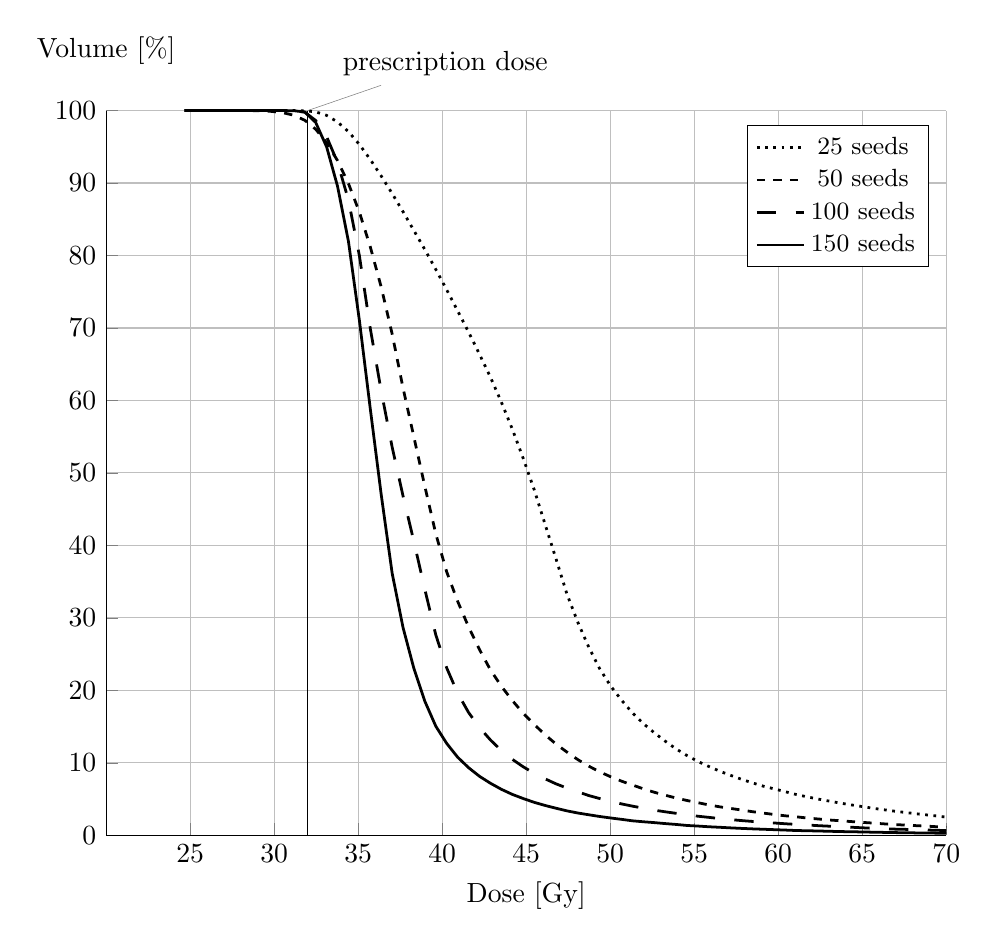
\begin{tikzpicture}
	\begin{axis}[%
		width=0.88\columnwidth,
		%height=0.8\columnheight,
		scale only axis,
		grid,
		xmin=20,
		xmax=70,
		xtick={25,30,35,40,45,50,55,60,65,70},
		xlabel style={align=center},
		xlabel={Dose [Gy]},
		ymin=0,
		ymax=100,
		ytick={0,10,20,30,40,50,60,70,80,90,100},
		ylabel={Volume [\%]},
		every axis y label/.style={
		    at={(ticklabel* cs:1.05)},
		    anchor=south,
		},
		axis x line*=bottom,
		axis y line*=left,
		%legend style={at={(0.03,0.97)},anchor=north west,draw=black,fill=white,legend cell align=left},
		legend style={font=\small},
		clip=false
		%enlargelimits=false
	]

\addplot [color=black,dotted,line width=1.0pt]
	table[row sep=crcr]{24.675 100.0 \\
25.325 100.0 \\
25.974999999999998 100.0 \\
26.625 100.0 \\
27.275 100.0 \\
27.925 100.0 \\
28.575 100.0 \\
29.224999999999998 100.0 \\
29.875 100.0 \\
30.525 100.0 \\
31.175 100.0 \\
31.825 99.9806142512947 \\
32.475 99.81814321452639 \\
33.125 99.33349949689367 \\
33.775000000000006 98.42790809308852 \\
34.425000000000004 97.09398395598511 \\
35.075 95.31880325311324 \\
35.725 93.24637440342666 \\
36.375 90.96254857976312 \\
37.025000000000006 88.55317695496045 \\
37.675000000000004 86.03118336148883 \\
38.325 83.42149233339795 \\
38.975 80.79426181838323 \\
39.625 78.07010255984196 \\
40.275000000000006 75.24532203421123 \\
40.925000000000004 72.35407608444801 \\
41.575 69.42775116083708 \\
42.22500000000001 66.36664912717973 \\
42.875 63.202156433760734 \\
43.525000000000006 59.7625707349045 \\
44.175000000000004 56.046968899720284 \\
44.825 52.00088620565509 \\
45.47500000000001 47.70371190931162 \\
46.125 42.90897006286521 \\
46.775000000000006 38.15392284472015 \\
47.425000000000004 33.28440739612469 \\
48.075 29.382333121013225 \\
48.72500000000001 25.951978731064273 \\
49.375 22.979497262916908 \\
50.025000000000006 20.601512088399012 \\
50.675000000000004 18.640782076490623 \\
51.325 16.883140860542618 \\
51.97500000000001 15.409823958939139 \\
52.625 14.139595853296042 \\
53.275000000000006 12.980143454540421 \\
53.925000000000004 11.912081013966972 \\
54.575 10.991719515910162 \\
55.22500000000001 10.180287462959376 \\
55.875 9.48609303313117 \\
56.525000000000006 8.836208886057955 \\
57.175000000000004 8.259252079352333 \\
57.825 7.716451115603682 \\
58.475 7.217960434610024 \\
59.12500000000001 6.763780036371357 \\
59.775000000000006 6.388988894735384 \\
60.425000000000004 6.00681270597358 \\
61.075 5.62094399364886 \\
61.725 5.295078789221524 \\
62.37500000000001 4.995061249734601 \\
63.025000000000006 4.7153525898437145 \\
63.675000000000004 4.443952107969389 \\
64.325 4.195629898363289 \\
64.97500000000001 3.9694628301346855 \\
65.62500000000001 3.728525667654417 \\
66.275 3.522667479021851 \\
66.925 3.3232712066243875 \\
67.575 3.1432606829322336 \\
68.22500000000001 2.961403897458621 \\
68.87500000000001 2.7989328606903174 \\
69.525 2.636461823922014 \\
70.0 2.4961459285312064 \\
	};
\addlegendentry{ 25 seeds};

\addplot [color=black,dash pattern=on 3pt off 3pt,line width=1.0pt]
	table[row sep=crcr]{24.675 100.0 \\
25.325 100.0 \\
25.974999999999998 100.0 \\
26.625 100.0 \\
27.275 100.0 \\
27.925 100.0 \\
28.575 100.0 \\
29.224999999999998 99.97733556955714 \\
29.875 99.88214496169712 \\
30.525 99.70082951815421 \\
31.175 99.35542359820498 \\
31.825 98.65917229500023 \\
32.475 97.42532070169077 \\
33.125 95.55777163319885 \\
33.775000000000006 93.09369475545078 \\
34.425000000000004 89.92248764788539 \\
35.075 85.98794252300439 \\
35.725 81.17945696024658 \\
36.375 75.63029781061601 \\
37.025000000000006 69.17184171161779 \\
37.675000000000004 61.68985993381987 \\
38.325 54.87693214269525 \\
38.975 48.0921082453198 \\
39.625 41.55659308281584 \\
40.275000000000006 36.314763609990486 \\
40.925000000000004 32.265989755677445 \\
41.575 28.73849780155025 \\
42.22500000000001 25.61080640043516 \\
42.875 22.807669643261868 \\
43.525000000000006 20.56117129776529 \\
44.175000000000004 18.59299215810707 \\
44.825 16.833325778523186 \\
45.47500000000001 15.29305108562622 \\
46.125 13.870631431032141 \\
46.775000000000006 12.583291781877524 \\
47.425000000000004 11.479080730701238 \\
48.075 10.433797198676398 \\
48.72500000000001 9.535379175921308 \\
49.375 8.753909614251395 \\
50.025000000000006 8.073976700965504 \\
50.675000000000004 7.462943656225919 \\
51.325 6.929876252209782 \\
51.97500000000001 6.408594352023934 \\
52.625 5.930828158288383 \\
53.275000000000006 5.524681564752278 \\
53.925000000000004 5.133946783917321 \\
54.575 4.793980327274376 \\
55.22500000000001 4.492090113775441 \\
55.875 4.180227550881646 \\
56.525000000000006 3.9209464666152947 \\
57.175000000000004 3.697021893839808 \\
57.825 3.479443361588323 \\
58.475 3.248266171071121 \\
59.12500000000001 3.0542586464802137 \\
59.775000000000006 2.8593445446715924 \\
60.425000000000004 2.6807488327818323 \\
61.075 2.5447622501246543 \\
61.725 2.3770454648474684 \\
62.37500000000001 2.247404922714292 \\
63.025000000000006 2.107792031186256 \\
63.675000000000004 2.0026290739313723 \\
64.325 1.8911200761524867 \\
64.97500000000001 1.7796110783736008 \\
65.62500000000001 1.6844204705135764 \\
66.275 1.575631204387834 \\
66.925 1.4750011332215223 \\
67.575 1.4006618013689318 \\
68.22500000000001 1.3236027378631976 \\
68.87500000000001 1.251076560446036 \\
69.525 1.1631385703277277 \\
70.0 1.0869860840397083 \\
	};
\addlegendentry{ 50 seeds};

\addplot [color=black,dash pattern=on 7pt off 7pt,line width=1.0pt]
	table[row sep=crcr]{24.675 100.0 \\
25.325 100.0 \\
25.974999999999998 100.0 \\
26.625 100.0 \\
27.275 100.0 \\
27.925 100.0 \\
28.575 100.0 \\
29.224999999999998 100.0 \\
29.875 100.0 \\
30.525 99.99909588174134 \\
31.175 99.9773970435333 \\
31.825 99.78572397269564 \\
32.475 98.62754848334163 \\
33.125 96.40070521224177 \\
33.775000000000006 92.8339586817956 \\
34.425000000000004 87.6452239952986 \\
35.075 79.96835586094662 \\
35.725 69.90913611500385 \\
36.375 61.27480674472221 \\
37.025000000000006 53.54911622440215 \\
37.675000000000004 46.79354459563311 \\
38.325 40.46833325799014 \\
38.975 33.872790561005374 \\
39.625 27.610867501469187 \\
40.275000000000006 23.062248542109305 \\
40.925000000000004 19.59314678359929 \\
41.575 16.92780615704534 \\
42.22500000000001 14.856471226436415 \\
42.875 13.146783599294787 \\
43.525000000000006 11.692057321097598 \\
44.175000000000004 10.477826499706161 \\
44.825 9.445323448307038 \\
45.47500000000001 8.545725780932147 \\
46.125 7.785362325392161 \\
46.775000000000006 7.0946159757696305 \\
47.425000000000004 6.511459698928619 \\
48.075 5.981646399349034 \\
48.72500000000001 5.478956647529497 \\
49.375 5.066678721576783 \\
50.025000000000006 4.677907870349442 \\
50.675000000000004 4.325301749468831 \\
51.325 4.016093305004294 \\
51.97500000000001 3.7349125265584737 \\
52.625 3.4627729306993356 \\
53.275000000000006 3.236743366032277 \\
53.925000000000004 3.0242755752452424 \\
54.575 2.8217530853035577 \\
55.22500000000001 2.625559423172551 \\
55.875 2.4673387279056103 \\
56.525000000000006 2.3027892048279917 \\
57.175000000000004 2.1617467564757473 \\
57.825 2.0234166628995074 \\
58.475 1.9040730527553003 \\
59.12500000000001 1.806428280819131 \\
59.775000000000006 1.6916052619682653 \\
60.425000000000004 1.5858234257040822 \\
61.075 1.496315718095927 \\
61.725 1.4158491930744541 \\
62.37500000000001 1.3245332489489625 \\
63.025000000000006 1.2512996699968355 \\
63.675000000000004 1.1862031553727226 \\
64.325 1.1084489851272545 \\
64.97500000000001 1.0334071696577911 \\
65.62500000000001 0.9637900637403372 \\
66.275 0.8968853125988878 \\
66.925 0.847158808372135 \\
67.575 0.8118981962840739 \\
68.22500000000001 0.7666922833506622 \\
68.87500000000001 0.7205822521585823 \\
69.525 0.6789928122598435 \\
70.0 0.6419239636544459 \\
	};
\addlegendentry{100 seeds};

\addplot [color=black,solid,line width=1.0pt]
	table[row sep=crcr]{24.675 99.99999999999999 \\
25.325 99.99999999999999 \\
25.974999999999998 99.99999999999999 \\
26.625 99.99999999999999 \\
27.275 99.99999999999999 \\
27.925 99.99999999999999 \\
28.575 99.99999999999999 \\
29.224999999999998 99.99999999999999 \\
29.875 99.99999999999999 \\
30.525 99.99999999999999 \\
31.175 99.9801560456411 \\
31.825 99.80246245433635 \\
32.475 98.35926577368872 \\
33.125 94.98940152437649 \\
33.775000000000006 89.5467460424841 \\
34.425000000000004 81.92937356244082 \\
35.075 71.03323862355117 \\
35.725 58.81477472601813 \\
36.375 46.97875794885672 \\
37.025000000000006 36.14666486267082 \\
37.675000000000004 28.633924141974475 \\
38.325 22.954945203626032 \\
38.975 18.46119153925946 \\
39.625 15.031795426870517 \\
40.275000000000006 12.655932891354349 \\
40.925000000000004 10.76173724800433 \\
41.575 9.320344563207506 \\
42.22500000000001 8.127903305822397 \\
42.875 7.173589500744148 \\
43.525000000000006 6.34014341767014 \\
44.175000000000004 5.638389031705227 \\
44.825 5.065620349073197 \\
45.47500000000001 4.543363550263835 \\
46.125 4.111306543994949 \\
46.775000000000006 3.7279574256979213 \\
47.425000000000004 3.366256257610608 \\
48.075 3.069498940152438 \\
48.72500000000001 2.826861498218554 \\
49.375 2.5896360438370993 \\
50.025000000000006 2.384882514770216 \\
50.675000000000004 2.195462950435214 \\
51.325 1.9916114192937355 \\
51.97500000000001 1.8608217201100439 \\
52.625 1.7435619898074235 \\
53.275000000000006 1.6100662968475172 \\
53.925000000000004 1.4910025706940875 \\
54.575 1.350290894330943 \\
55.22500000000001 1.2682090831191088 \\
55.875 1.1716953051007983 \\
56.525000000000006 1.0986334731430119 \\
57.175000000000004 1.0174536598565824 \\
57.825 0.9443918278987958 \\
58.475 0.8803499751950571 \\
59.12500000000001 0.825328101745366 \\
59.775000000000006 0.7694042303702702 \\
60.425000000000004 0.714382356920579 \\
61.075 0.6530464979930546 \\
61.725 0.6214765706038876 \\
62.37500000000001 0.588102647363911 \\
63.025000000000006 0.5493167365715059 \\
63.675000000000004 0.509628827853696 \\
64.325 0.4843728859423624 \\
64.97500000000001 0.45550895232940963 \\
65.62500000000001 0.4230370270148378 \\
66.275 0.39507509132728996 \\
66.925 0.3662111577143372 \\
67.575 0.3481711992062418 \\
68.22500000000001 0.3238172552203129 \\
68.87500000000001 0.30938528841383656 \\
69.525 0.28773733820412206 \\
70.0 0.26518739006900277 \\
	};
\addlegendentry{150 seeds};

\draw ({axis cs:32,0}|-{rel axis cs:0,1}) -- ({axis cs:32,0}|-{rel axis cs:0,0});
\node[coordinate,pin=above right:{prescription dose}] at (axis cs:32,100) {};

\end{axis}
\end{tikzpicture}% 
			\caption{Dose Volume Histograms of the PTV for different numbers of seeds.}
			\label{fig:LPSW_DVH_numberOfSeeds}
		\end{figure}


\begin{acknowledgement}
Please insert acknowledgments of the assistance of colleagues or similar notes of appreciation here.
\end{acknowledgement}

\def\acknowledgementname{Funding}
\begin{acknowledgement}
Please insert information concerning research grant support here
\end{acknowledgement}

%\bibliographystyle{...}
%\bibliography{...}

\begin{thebibliography}{9}
%---------------------------------------------------------------------------------------------------------------------%
% The Reference list at the end of the manuscript should be in alphanumerical order (see samples below).							%
%---------------------------------------------------------------------------------------------------------------------%

% Books


\bibitem{1}
Koza, John R. Genetic Programming. 3rd ed. Cambridge: MIT Press 1992.

\bibitem{2}
Williams, H. Paul Model Building in Mathmetical Programming, 4th ed., 1999.

\bibitem{3}
Schlaefer, A. and Schweikard, A. Stepwise multi-criteria optimization for robotic radiosurgery. Med. Phys. 2008.



\end{thebibliography}
\end{document}
